\section{Energy Storage and Arbitrage}
Using mixed integer programing techniques, form and solve a mathematical model of economic
dispatch on an electrical grid capable of energy storage with a diverse set of power generation assets.

\subsection{Motivation}
The current structure of the electrical grid requires an exact balance of supply and demand,
while being held to a very high standard of reliability. The Independent System Operator is in charge of
maintaining the reliability of the grid while also minimizing the cost of power generation by choosing
which generators to dispatch.[4] Introducing energy storage to the electrical grid gives the ISO an extra
degree of flexibility in operating the grid. This can lead to increased reliability of the grid and lower total
cost of power generation. \\

This model looks at a multiple day time frame, in which the electrical demand is met at all time
periods with the lowest possible cost to the system. It is focused on the possible economic gains of
having the capability to store energy on the electrical grid. Storing energy can help deal with
instantaneous changes in electrical demand, without the need to dispatch expensive generators in order
to meet demand. It also has potential to help with grid congestion, which can lead to high variability in
spot-prices on wholesale electrical markets. Due to grid congestion, it is possible for wholesale markets
to have negative prices at certain buses on the grid. This means that there is a possibility that you would
get paid to store energy, and then also get paid when you dispatched it. However, it is not necessary for
the markets to have negative prices in order to operate energy storage for a profit. With the high
variability of spot prices, it would be possible to take advantage of any significant price differentials at a
given bus over time. Lastly, as intermittent power generation (renewables such as wind power) become
more prevalent on the electrical grid, it may become necessary to store energy in order to operate these
power generation assets in an efficient manner. \\

Since there are many reasons why energy storage is becoming important to the electrical grid,
one must look at the options available to store energy. Certain power generation assets have a natural
form to store energy for later use. The simplest version is a hydro-dam with the capability of pumped
storage. When the energy markets are in need of energy, the hydro-dam lets the turbines spin to
produce energy to sell to the grid. And when the energy markets have too much energy, the hydro-dam
can pump water back into the reservoir for later use. This type of energy storage is able to achieve
around 70% to 85% round trip efficiency.[5] Another generation asset that has a natural form for energy
storage is concentrating solar thermal energy. Using mirrors to concentrate solar irradiation, it is
possible to heat a fluid for the eventual end-use of generating steam to spin turbines. This energy can
be stored in molten salt reservoirs for use on demand. [6] The last practical energy storage is batteries.
With the introduction of plug-in hybrids and electrical vehicles to the car market, the electrical grid is
going to have increased electrical demand, but also the possibility to leverage the energy storage of the
vehicles for the electrical grid. While the cars have just recently been introduced, there is relatively no
energy storage currently available. However, as these cars become main-stream and are deployed in
large numbers, they could play a significant role in the capabilities for the electrical grid to store energy.
Lithium-ion batteries can reach round-trip efficiencies of 92%.[2] This comes with a steep upfront cost.
However, as these are purchased as a package with the electrical vehicle, any money that could be
made from using the batteries as energy storage for the grid would be a net positive for anyone who
owns an electrical vehicle. This comes with plenty of logistical problems, but the positives may
outweigh the negatives.  \\

With today’s technology, there are multiple ways of efficiently storing energy for use on the
electrical grid. Due to how the grid operates, there are many avenues that using energy storage could
benefit both the consumer of power through lower energy prices and those operating energy storage
for economic gain. Given that there are multiple forms this energy storage may take, no assumptions
will be made on the financial cost of energy storage, only that it comes at a cost to efficiency. This
means that even though it will be cheaper to meet demand, total energy production will have to
increase. \\

As there are many ways that energy storage can be implemented on the electrical grid, it is
important to start looking at the effects this may have. What follows will be a formulation of a
minimum cost dispatch model of an electrical grid. First, the main ideas of the formulation will be
recognized, and then the mathematical formulation will be shown. Then, data must be formed for the
problem instance. All of the data used is randomly generated, with an attempt to capture realities of
the electrical grid. The random data will help ensure that the methodologies of studying this problem
are robust to separate data instances. Once the data has been formed, an attempt will be made to solve
the model optimally. As size of this problem becomes unwieldy as the number of nodes and time
periods increase, different methods will be employed to try to speed up the solve time. The results of
the model will then be explained, as will the success of the various methods employed. The conclusion
will then sum up the significant points of this report.

\subsection{Formulation of Energy Storage Problem}
The basis for this model is the DC power flow model. It is an approximation to the true nonlinear
power flow on an electrical grid. It is reliable for active power flow analysis as long as the
following assumptions are met.[3]
\subsection{Assumptions}
\begin{itemize}
\item Voltage angle difference are small, ( $sin( \theta ) \approx \theta $ )
\item Line resistance can be neglected, i.e. a lossless line
\item Flat voltage profile, avoid deviation from predefined value
\end{itemize}
These assumptions are decent for a real power grid, and results in an error of under 5\%.[3] The
following equations form the DC power flow model. $p_i$ is the active power injected into the grid at
node $i$.  $s_{ij}$ is the line susceptance for power flow on a given line. $\theta_i$ is the voltage angle at node $i$. $\cV$ is
the set of all verticies (nodes).  $d_i$ is the demand for node $i$. 
\begin{align*}
	p_i = \sum_j s_{ij} ( \theta_i - \theta_j ) \\
	p_{i,gen} - d_i  = p_i
\end{align*}


For energy storage to be viable, there must be significant difference in the marginal price of
energy over time. The two main reasons for the difference in marginal price are grid congestion and the
limited capabilities of generation assets. This study focuses primarily on the effect of having differences
in the capabilities of generation assets. The generators will be modeled with both a fixed cost for
operating and a per-unit cost for each unit of electricity generated. The other critical factor to model is
the limited range of dispatch of a generator over time. This is to represent the fact that a coal plant
cannot ramp up production from no energy produced to full capacity in an arbitrarily small amount of
time. The first constraint enforces an upper capacity as well as the binary variable $y$, which represents
whether the generator is on or off. The second constraint represents the range of dispatch over time.  $\alpha$ is a parameter that describes the flexibility of power output from a given generator.  The higher $\alpha$ plants are able to better match the unpredictable, short term fluctuation in demand. 
\begin{align}
	p_{git} \leq y_{git} u_g  \\
	\left|  p_{git} - p_{gi \rho (t)}  \right|  \leq  \alpha_g 
\end{align}
where $\rho (t)$ is the predecssor to time t.  The range of dispatch constraints give a generator an effective start-up and turn-off time to ramp up and down from full capacity. An estimate of this time is represented by the following. 
\begin{equation*}
	t_{eff} = \frac{u_g}{\alpha_g}
\end{equation*}

Lastly, to model the capability of energy storage, non-negative variables $p_{stor}$ and $d_{stor}$ represent the
amount of stored energy dispatched and the amount of energy stored, respectively. Then with $e$ representing the amount of energy currently stored, the following equation links the energy storage over time. $\eta$ is the round trip efficiency of energy storage.
\begin{equation}
e_{t} = e_{\rho (t)} - p_{stor, \rho (t)} + \eta d_{stor, \rho (t)}
\end{equation} 

Finally, the DC power flow is adapted to include a load of energy stored and a supply
of stored energy dispatched. The complete mathematical model is in the appendix.

\subsection{Forming Problem Instance Data}
Two major factors determining the difficulty of the problem instance are the number of nodes in
the grid and the number of time periods. To make the problem of reasonable size, 14 nodes and 72
time periods are used. This means there are approximately N*T (1008) binary variables and 6*N*T
(6048) continuous variables. There are three main components to the rest of the data for the problem.
They are electrical demand, grid topology, and the power generation assets. All of the data is randomly
generated in a way to represent what a real world example would entail. First, the electrical demand
will be looked at. Following is the grid topology and finally the power generators.
Electrical demand varies both daily and seasonally. Since this is only a multi-day model, just the
daily variation needs to be accounted for. This is done for each node by the following.

\begin{itemize}
\item Randomly generate a base-load consumption number, that is the minimum demand
over a full 24 hour period.
\item Perturb a sine wave function to represent how the demand peaks. Peak power is the
maximum demand over the 24 hour period. The sine wave has a 24 hour period, and is
then scaled according to a randomly generated peak demand number.
\item For each time period, a coin is flipped to see if there is an extra instantaneous demand.
If so, a random number is scaled to represent a one-time demand to the system.
\item Finally, the base-load, peak demand function, as well as the random single period
demands are added together. The following is a sample of a one day demand scenario.
\end{itemize}

\begin{figure}[h]
\centering
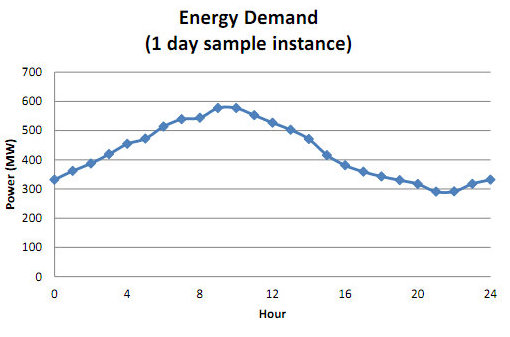
\includegraphics[width=4in]{random_demand}
\caption{An example of random demand scenario for a 24 hour day}
\label{fig:random_demand}
\end{figure}

The real world electrical grid is a graph with sparse edges connecting the nodes. For a given
interconnected grid, there are normally no islands. That is, the set of connected components of the
graph is all the nodes. For each node, the following is done to form edges.
\begin{itemize}
\item Flip coin for every other node and connect the edge with a given probability. This edge
is given a random electrical susceptance number, with an upper and lower bound. This
number is largely responsible for how electricity is allowed to flow on the network. An
analog would be the diameter of a pipe for a gas/fluid pipeline.
\item If no edges were connected, a random node is picked to connect
with an edge. This is then given a random electrical susceptance
number.
\end{itemize}

\begin{figure}[h]
\centering
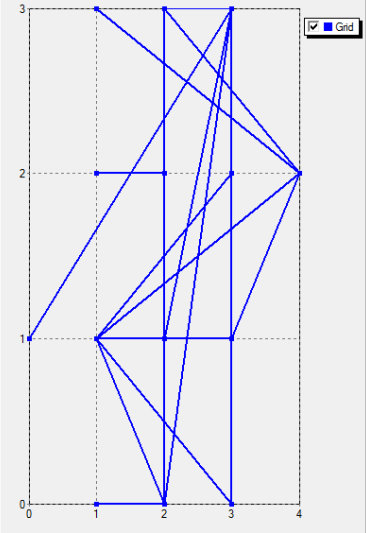
\includegraphics[width=2in]{grid_instance}
\caption{An example of a grid instance}
\label{fig:grid_instance}
\end{figure}

Since this does not guarantee the lack of islands, an attempt was made to
visualize the grid. In practice, an island was rarely seen. Here is an example of one
of the grid topologies used. Since this is a lossless network, there is no significance
to the nodes in relationship to some relative geography. The output of each model
graphs the grid topology as well as showing the total number of edges in the graph.
While it was a goal to create a relatively sparse network, the number of lines as
well as the electrical susceptance of each line is critical in determining whether the
problem is feasible. The probabilities used to generate the grid were a
compromise between creating a sparse grid and one that is usually feasible.  \\

The last set of data is that for the power generators. This data was hand-coded in order to
represent a scenario in which energy storage is useful. This was done be creating a set of cheaper
generation assets that have low range of dispatch as well as a set of more expensive generation assets
that have a high range of dispatch. Generators can be classified into two categories, base load power
plants and peaking power plants. The set of generator data chosen was an attempt to capture the
characteristics of the real world generators of a coal plant (relatively cheap per-unit cost with low range
of dispatched, base load power plant) compared to a natural gas plant (relatively expensive with high
range of dispatch, peaking power plant). Lastly, each node is randomly assigned one of the six types of
generators, or no generator. 

\begin{table}
\caption{Set of Possible Generator Parameters}
  \begin{tabular}{ l l }
Generator type: 1  	&	 Generator type: 2	\\
\hline
Fixed Cost: 30, Variable Cost: 3 	&	Fixed Cost: 50, Variable Cost: 5 	\\
Change in production per time: 10  	&	Change in production per time: 30 	\\
Max production per generator: 125 	&	Max production per generator: 75   	\\
Effective start-up time: 12.5  		&	Effective start-up time: 2.5	\\
  &    \\
 Generator type: 3			&	 Generator type: 4	\\
\hline
 Fixed Cost: 60, Variable Cost: 2	&	  Fixed Cost: 90, Variable Cost: 3.5	\\
Change in production per time: 8  	&	Change in production per time: 37	\\
Max production per generator: 300 	&	Max production per generator: 200	\\
Effective start-up time: 37.5 		&	Effective start-up time: 5.4	\\
	&	\\
Generator type: 5			&	Generator type: 6	\\
\hline
 Fixed Cost: 100, Variable Cost: 1 	&	Fixed Cost: 150, Variable Cost: 2	\\
Change in production per time: 5	&	Change in production per time: 45	\\
Max production per generator: 600 	&	Max production per generator: 400	\\
Effective start-up time: 120		&	Effective start-up time: 8.9 	
  \end{tabular}
\end{table}
\subsection{Improving the bounds}
\subsubsection{Lagrangian Relaxation}
The above formulation has several hard constraints. In order to speed up the solve as well as
possibly finding a good lower bound, Lagrangian relaxation was performed on two of the constraints
separately. The first constraint that could be seen as the hardest is the strict equality of energy balance
at each node. 
\begin{equation}
\sum_{g \in \cG} P_{git} - S_{it} - L_{it} - P_{it} = 0
\end{equation}
Since it is an equality constraint, a free weight $\lambda$ is assigned to penalize not meeting this
constraint exactly. The objective function then becomes the following. 
\begin{equation}
\mbox{ minimize }  \sum_{t \in \mathcal{T}} \sum_{i \in \mathcal{I}} \sum_{g \in \mathcal{G}} \biggl[  F_g Y_{git} + V_g P_{git} \biggr]  + \lambda \sum_t \sum_i \sum_g \biggl[   P_{git} - S_{it} - L_{it} - P_{it}  \biggr]
\end{equation}

This was a bad idea. Since the grid was capable of storing or dispatching energy, the program
either drove energy storage or stored energy dispatch arbitrarily high in order to take advantage of
either a positive or negative weight. The program ultimately ended up producing no energy for the
nodes to consume.  \\

The other constraint that can be very restrictive is the range of dispatch constraint. This
enforces strong conditions on what any given generator is able to do from any given time period to the
next. 
\begin{align}
	-P_{gi(t+1)} + P_{git} - \alpha_g \leq 0 \\
	P_{gi(t+1)} - P_{git} - \alpha_g \leq 0
\end{align}

Then assigning each constraint a non-negative weight $\lambda$ and $\mu$, the constraints can be moved
into the objective. The following objective penalizes violation of the constraints. 
\begin{equation}
 \sum_{t \in \mathcal{T}} \sum_{i \in \mathcal{I}} \sum_{g \in \mathcal{G}} 
	\biggl[  F_g Y_{git} + V_g P_{git} + \lambda ( -P_{gi(t+1)} + P_{git} - \alpha_g )  + \mu ( P_{gi(t+1)} - P_{git} - \alpha_g ) \biggr] 
\end{equation}
Equivalently,
\begin{equation}
 \sum_{t \in \mathcal{T}} \sum_{i \in \mathcal{I}} \sum_{g \in \mathcal{G}} 
	\biggl[  F_g Y_{git} + V_g P_{git} + (\mu - \lambda) P_{gi(t+1)} + (\lambda - \mu) P_{git} - (\lambda + \mu) \alpha_g
	 \biggr] 
\end{equation}
This didn’t work either. The lower bound was much worse than those found by the solver. The
symmetric nature of the constraints led to an awkward penalty function. The objective was
systematically lowered by the negatively weighted values. \\

Next, an attempt was made to relax the range of dispatch constraint while not penalizing the
objective function. This attempt led to a much better lower bound (one instance gave a lower bound
within 2\% ). However, the problem still appeared to be computationally difficult. The solver was not
able to consistently find a proven optimal solution of the relaxation in significantly less time.
The source code for the main function in the attempt to find a decent relaxation is in the
appendix.

\subsubsection{Heuristic}
In solving the model, it became readily apparent that finding feasible solutions is a hard part of
the problem. In the various solves performed, it was seen that only around 5 to 10 feasible solutions
were found, and never more than 20. Because of this, a heuristic which develops feasible solutions
could be useful. Following will be an outline of a possible algorithm that may develop quality feasible
solutions. However, the heuristics has not been implemented, so the quality of the heuristics is
unknown. \\

Since the model is capable of storing energy, an obvious solution would be to generate the same
amount of energy each time period, and then redistribute the energy through storage based on the
given demand in a time period. After this solution is found, iteratively improve it by finding time periods
in which the marginal cost of electricity is lower than the average cost of electricity for the base
scenario. Then, increase production at that time period, and lessen the constant production over time
by an equivalent amount. This is somewhat complicated due to the efficiency of energy storage not
being equal to 1 (we live in the real world). \\

\begin{algorithm}
\caption{Hueristic for Unit Commitment with Energy Storage}
\begin{algorithmic}
\REQUIRE $ \eta, \epsilon $
\STATE $ k \gets 0 $
\STATE Find the constant production needed per time period to satisfy total demand  \\
	-This can be done iteratively, first find average electrical demand \\
	- For each time t, look at difference between demand and average electrical demand \\SS
	-Scale the stored energy by the efficiency, and look at difference from dispatched energy \\
	-Divide this difference by T (total periods) and add this value to average electrical demand  \\
	-Repeat until scaled stored energy is arbitrarily close to dispatched energy
\STATE Find the optimal dispatch for this demand 
\WHILE{ $ \left| c_{eff} - c \right| \leq \epsilon  $}
	\STATE $k \gets k + 1 $

	\STATE Look at time periods in which demand is greater than constant production \\
	-Effective marginal cost is then average cost divided by efficiency, because energy is being
	dispatched from storage to meet the last unit of demand  \\
	-Then calculate marginal cost from increasing generator production at that time period \\
	-If actual marginal cost is less than effective marginal cost, increase production at that time
	period until the two become close  \\
	-Take the energy displaced from increased production and divide by efficiency to find actual
	energy displaced  \\
	-Divide this figure by T, and lower constant production by this amount
\ENDWHILE

\end{algorithmic}
\end{algorithm}

\subsection{Results}
The model as formed proved to be hard to solve in a timely manner. The large number of
variables and tough constraints made finding feasible solutions difficult. The following table summarizes
the results of five separate data runs. Then, an explanation of the results will follow. \\

\begin{table}
\caption{Results from Five Trial Runs}
  \begin{tabular}{ l c  l l l l l l l l l l l }
Trial  	&  Energy  	&  \#  of	&	Avg. Unit	&		Solve	&	Optimality	&	Nodes \\
 \#     	&  Storage 	&  Lines	& 	Cost		&		Time (s) &	Gap (\%)	&	Processed \\
1	& Yes		& 22		&  	1.32		&	 1000	&	 .0135	&	 106557  \\
1	& No	& 22 	& 1.60   &  1000   &    .0391   &   139349  \\
2	& Yes	& 28	& 1.19  & 1000    &    .0131   & 154608  \\
2	&  No   &  28  	& 1.55  & 1000   &  .0226  &   172197  \\
3 	& Yes   & 22   	& 1.85  & 1000  &   .0040  &   64067   \\
3	&  No   & 22   	& 1.95  & 1000  & .0104   &  145837  \\
4	&  Yes  & 27     & 1.76 &  20.7  &  1e-5   & 264	\\
4	&   No  &  27	& 1.90  & 1000  & .0057 & 152631 \\
5	&  Yes & 27 	& 1.30  & 1000  & .0133 & 24002 \\
5	&  No & 27 	& 1.41  & 1000 &  .0311 & 129012
  \end{tabular}
\end{table}

As can be seen, almost all of the runs hit the time limit before proving an optimal solution. A
typical run started out with large gains in both feasible solutions as well as improved lower bounds for
the beginning iterations. As the number of iterations increased, the model begins to stagnant and
reduces to an almost complete enumeration of feasible solutions. However, even without proven
optimal solutions, a number of conclusions can be drawn from the results of these runs.	\\

First, looking at the computational difficulty of solving the problem with versus without energy
storage, the problem is easier with the capability of energy storage. This is not surprising. When the
model is able to store energy, the range of dispatch constraints become less important. Since the grid
can store energy, it is not necessary for the model to meet demand exactly at every time period.	\\

Typically, the model finds an optimal power output of the generators and tries to operate at that level
for the majority of the time. Then, at a cost to efficiency, the model redistributes energy from the low
demand time periods to the high demand time periods. \\

Next, the difference in average unit cost of electricity is important to note. While the generator
data is not from the real world and may be exaggerated to some extent, the model was able to
consistently find improvements in total cost of dispatch. While this does not prove that energy storage
will be economically feasible in the real world, it is strong evidence to suggest that the situation should
be investigated further.  \\

Lastly, a note should be made on solve , which was able to find an optimal solution. The total
energy demand was less than usual for this problem. As such, the model was able to operate a cheap
generator constantly, and redistribute the energy without worries of a cheaper solution.

\subsubsection{Future Work}
The problem this study focused on is one in which there is no uncertainty. The demand is
known for all time periods, as well as the availability of generators and storage capabilities. An
interesting extension of this would be to look at the problem from ISO’s perspective. That is, current
demand is known and there is a probability distribution of future demand. Then, the ISO’s problem
would be to minimize the cost of current generation dispatch as well as the expected value of future
generation dispatch. This would be a stochastic programming model. It would help shed light on how
the ISO is supposed to operate when they have the capability to store and/or dispatch stored energy
now, while also minimizing the expected value of the future cost of power generation.	\\

Also, other work could be done on this model to help quantify the real economic benefits of
energy storage. While this model shows that energy storage could play a large role in decreasing total
cost of electrical generation, no attempt was done to use real world data. A real world grid topology as
well as a set of generating assets for that given grid would be necessary to put real world numbers into
this framework. Energy storage would also need to be modeled more precisely. That is, there may be
some fixed cost for constructing the storage capabilities, as well as possible operating and maintenance
cost. Then, the model would more accurately show the potential economic benefits of being able to
store energy on an electrical grid. To counter the complexity of the problem, a single day model could
be used along with the constraints that the energy stored at the beginning of the day is equal to that
stored at the end of the day.

\subsubsection{Conclusion}
The model formed for this study was able to effectively show that this situation is worth further
study. While it most certainly has its shortcomings, it is able to show the major factors that play into the
dynamics of energy storage on the electrical grid. The main factor in determining the effectiveness for
energy storage is a difference in marginal prices over time. This study looked at how the range of
dispatch of generators can lead to these price differences. Since the figures used for the generator data
were hypothetical, no conclusion can be made to the level of actual economic gains possible of using
energy storage. However, it is probable that due to the pervasiveness of electricity in our world, there
are many situations in which energy storage could be operated for economic benefits.  \\

The major downside to this model is complexity. Even with a small grid size of 14 nodes, it took
too long to solve the problem optimally. While the relaxation approaches attempted were not helpful,
the heuristic suggested could prove useful to finding feasible solutions. Also, in the future work section
a note was made that the study need not be multiple day, only single day. The daily variation in
electrical demand is what energy storage is capable of smoothing. So, with a simple constraint that the
amount of energy stored at the beginning of the day is equal to that of the end of the day, only 24 time
periods are needed, versus the 72 used in this model. Also, the model used random data, which could
cause the problems to be more difficult than a real world instance might be. Lastly, the model is not
made to be used as an operation tool for operators of the grid, but to show the economics of energy
storage on the grid. As such, the time to solve the model is of less importance.

\subsubsection{Wholesale Market}
       	 Proper integration of energy storage on the electric grid can lead to stable wholesale electricity prices with increased reliability of the grid. Energy storage 	will be vital in the transition to increased de-centralized, intermittent generation from alternative energy sources such as wind and solar.  \\

\begin{figure}
\centering
      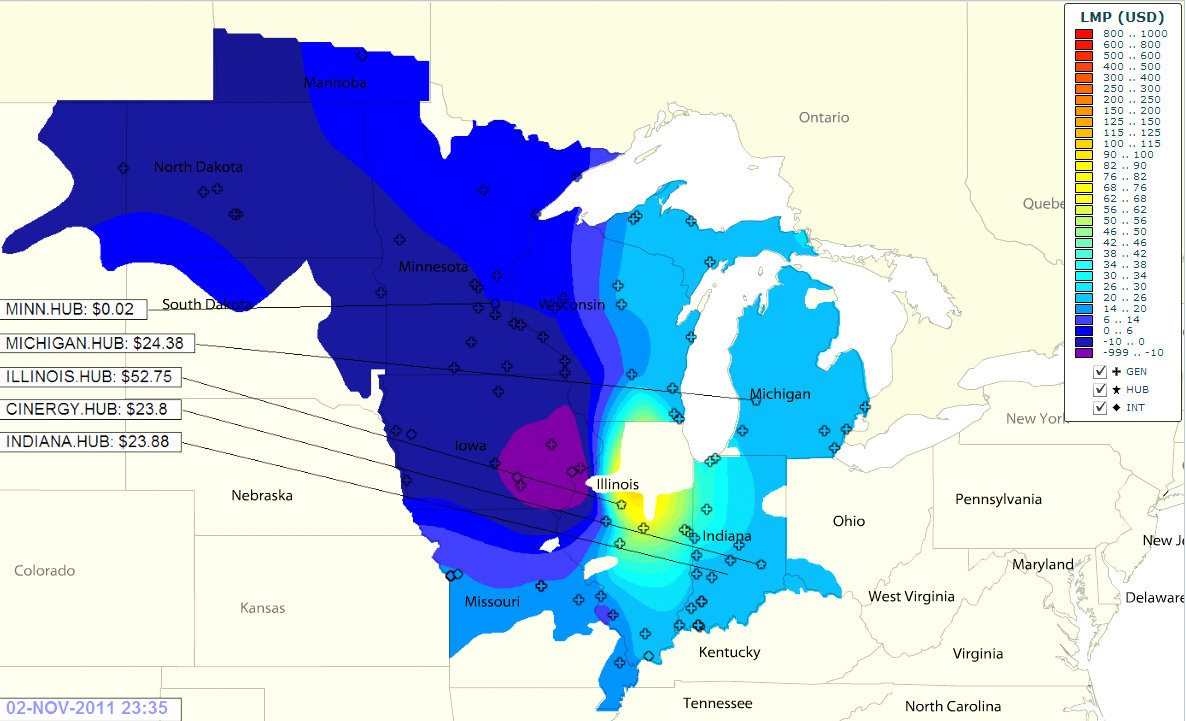
\includegraphics[width=5in]{lmp}
     \caption{Locational Marginal Pricing}
\end{figure}


Wholesale market:  
      		The sale of wholesale electricity is broken into three groups; long term contracts, day-ahead unit commitment, and the real time market.  Wind is typically structured with long term contracts, called Power Purchase Agreements, which settle on a fixed, long term, sale price.  Everyday, our indepent system operator create a unit commitment plan based on forecast for energy consumption at lowest cost.  The final real time market makes up for any discrepancy from forecast, and typically high cost units with fast response time are dispatched.


\subsubsection{Example Output }

\begin{figure}[h]
\centering
 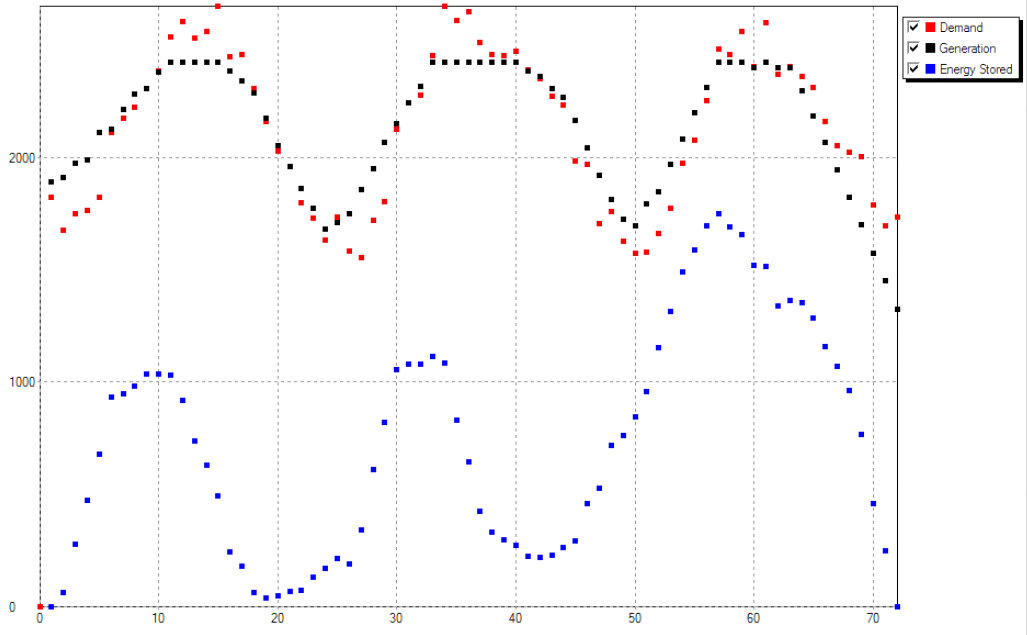
\includegraphics[width=5in]{mosel_graph_storage}
 \caption{Graph of load served, power produced, at stored energy}
\end{figure}


In order to operate storage assets in the real time market effectively, stochastic models accounting for a range of possible future scenarioes would need to be used.  The computational difficulty of this problem, even on small grids is time consuming, which will increase drasticly with even the most simple stochastic version.  To be able to solve in a timely manner, specialized algorithms will be needed along with significant computational resources. 

\begin{longtable}{ |  l  |  l  | }
\caption[Mosel Example Output]{Mosel Example Output}  \\
\hline
No Energy Storage Allowed &  Energy Storage Capacity: 1750 \\
\hline
Number of nodes: 14 & Number of nodes: 14 \\
Number of lines: 21 & Number of lines: 21 \\
Duration: 72 hours & Duration: 72 hours \\
\hline
Total Energy Consumed: 98220.2  &  Total Energy Consumed: 98220.2 \\
Total Energy Produced: 98220.2  &  Total Energy Produced: 100106  \\
Total Cost of Energy Produced: 164832  &  Total Cost of Energy Produced: 121706  \\
Per Unit Cost of Energy: 1.67818  &  Per Unit Cost of Energy: 1.21577 \\
  &  Energy Storage Efficiency: 0.9 \\ 
  &  Total Stored Energy: 23450 \\
\hline
	
Generator type: 1			&	Generator type: 1		\\
\hline
Fixed Cost: 30, Variable Cost: 3	&	Fixed Cost: 30, Variable Cost: 3	\\
Change in production per time: 10	&	Change in production per time: 10	\\
Max production per generator: 125	&	Max production per generator: 125 	\\
Number Deployed: 2			&	Number Deployed: 2			\\
Energy Produced: 2717.65		&	Energy Produced: 0			\\
Avg. Production per unit time: 37.7451&	Avg. Production per unit time: 0	\\
Variability in generation: 4.67676	&	Variability in generation: 0 	\\

\hline
Generator type: 2			&	Generator type: 2	\\
\hline
Fixed Cost: 50, Variable Cost: 5	&	Fixed Cost: 50, Variable Cost: 5	\\
Change in production per time: 30	&	Change in production per time: 30	\\
Max production per generator: 75	&	Max production per generator: 75	\\
Number Deployed: 3			&	Number Deployed: 3	\\
Energy Produced: 1402.12		&	Energy Produced: 0	\\
Avg. Production per unit time: 19.4739&	Avg. Production per unit time: 0	\\
Variability in generation: 6.07023	&	Variability in generation: 0	\\

\hline
Generator type: 3			&	Generator type: 3	\\
\hline
Fixed Cost: 60, Variable Cost: 2	&	Fixed Cost: 60, Variable Cost: 2	\\
Change in production per time: 8	&	Change in production per time: 8	\\
Max production per generator: 300	&	Max production per generator: 300	\\
Number Deployed: 2			&	Number Deployed: 2			\\
Energy Produced: 4166.09		&	Energy Produced: 0	\\
Avg. Production per unit time: 57.8624&	Avg. Production per unit time: 0	\\
Variability in generation: 6.41265	&	Variability in generation: 0	\\

\hline
Generator type: 4			&	Generator type: 4	\\
Fixed Cost: 90, Variable Cost: 3.5 	&	Fixed Cost: 90, Variable Cost: 3.5	\\
Change in production per time: 37	&	Change in production per time: 37	\\
Max production per generator: 200	&	Max production per generator: 200	\\
Number Deployed: 0			&	Number Deployed: 0	\\
Energy Produced: 0			&	Energy Produced: 0	\\
Avg. Production per unit time: 0	&	Avg. Production per unit time: 0	\\
Variability in generation: 0		&	Variability in generation: 0	\\

\hline
Generator type: 5			&	Generator type: 5	\\
\hline
Fixed Cost: 100, Variable Cost: 1	&	Fixed Cost: 100, Variable Cost: 1	\\
Change in production per time: 5	&	Change in production per time: 5	\\
Max production per generator: 600	&	Max production per generator: 600	\\
Number Deployed: 3			&	Number Deployed: 3			\\
Energy Produced: 76032.8		&	Energy Produced: 100106		\\
Avg. Production per unit time: 1056.01&	Avg. Production per unit time: 1390.37	\\
Variability in generation: 1.35824	&	Variability in generation: 1.43515	\\

\hline
Generator type: 6			&	Generator type: 6	\\
\hline
Fixed Cost: 150, Variable Cost: 2	&	Fixed Cost: 150, Variable Cost: 2	\\
Change in production per time: 45	&	Change in production per time: 45	\\
Max production per generator: 400	&	Max production per generator: 400	\\
Number Deployed: 1			&	Number Deployed: 1	\\
Energy Produced: 13901.5		&	Energy Produced: 0	\\
Avg. Production per unit time: 193.076&	Avg. Production per unit time: 0	\\
Variability in generation: 9.44763	&	Variability in generation: 0	\\


\hline
Performance of Solve			&	Performance of Solve	\\
\hline
Stop Status: Time Limit Hit		&	Stop Status: Solution is Optimal	\\
Time: 500.483				&	Time: 12.364		\\
Nodes Processed: 90418		&	Nodes Processed: 409		\\
Objective Value: 164832		&	Objective Value: 121706		\\
Best Bound: 160689			&	Best Bound: 121706		\\
Relative Optimality Gap: -0.0251332	&	Relative Optimality Gap: 0	\\
\hline
\end{longtable}


\subsection{Storage Options}
	Good options include Batteries, Electric Vehicles, Pumped Hydro, Thermal Mediums, and Compressing Gas  \\
Xcel's prototype
\begin{figure}[h]
\centering

\includegraphics[width=2.5in]{battery}
\caption{Xcel's 1 MW energy storage using sodium sulfur batteries}
\end{figure}

Optimal Siting:	Using historic pricing data, locations with large price volatility is ideal for storage opportunities.  Thus, it may be possible to lower the cost of an electric vehicle, in return for using the batteries within to take advantage of market opportunities.
 